\begin{figure}[tb]
\centering
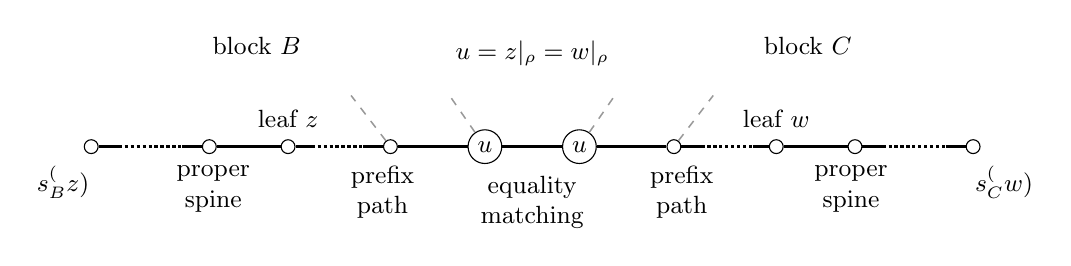
\begin{tikzpicture}[
  x=1cm,y=1cm,font=\small,
  vertex/.style={circle,draw,fill=white,inner sep=0pt,minimum size=5pt},
  root/.style={circle,draw,fill=white,inner sep=2pt},
  route/.style={line width=1.15pt},
  possible/.style={line width=.55pt,black!40,dashed}
]
  \node[vertex] (sB) at (-5.6,0) {};
  \node[vertex] (cB) at (-4.1,0) {};
  \node[vertex] (lB) at (-3.1,0) {};
  \node[vertex] (pB) at (-1.8,0) {};
  \node[root] (rB) at (-.6,0) {\(u\)};
  \node[root] (rC) at (.6,0) {\(u\)};
  \node[vertex] (pC) at (1.8,0) {};
  \node[vertex] (lC) at (3.1,0) {};
  \node[vertex] (cC) at (4.1,0) {};
  \node[vertex] (sC) at (5.6,0) {};
  \draw[route] (sB)--(-5.25,0) (-4.45,0)--(cB)--(lB);
  \draw[route,densely dotted] (-5.25,0)--(-4.45,0);
  \draw[route] (lB)--(-2.8,0) (-2.15,0)--(pB)--(rB);
  \draw[route,densely dotted] (-2.8,0)--(-2.15,0);
  \draw[route] (rB)--(rC)--(pC)--(2.15,0) (2.8,0)--(lC)--(cC);
  \draw[route,densely dotted] (2.15,0)--(2.8,0);
  \draw[route] (cC)--(4.45,0) (5.25,0)--(sC);
  \draw[route,densely dotted] (4.45,0)--(5.25,0);
  \draw[possible]
    (rB)--(-1.05,.65)
    (pB)--(-2.3,.65)
    (rC)--(1.05,.65)
    (pC)--(2.3,.65);
  \node[above] at (-3.5,1.05) {block \(B\)};
  \node[above] at (3.5,1.05) {block \(C\)};
  \node[below,anchor=north east] at (-5.5,-.12) {\(s_B^\eps(z)\)};
  \node[below,align=center] at (-4.05,-.12) {proper\\spine};
  \node[above] at (-3.1,.12) {leaf \(z\)};
  \node[below,align=center] at (-1.9,-.12) {prefix\\path};
  \node[below,align=center] at (1.9,-.12) {prefix\\path};
  \node[above] at (3.1,.12) {leaf \(w\)};
  \node[below,align=center] at (4.05,-.12) {proper\\spine};
  \node[below,anchor=north west] at (5.5,-.12) {\(s_C^\eps(w)\)};
  \node[below,align=center] at (0,-.25) {equality\\matching};
  \node[above] at (0,.9) {\(u=z|_\rho=w|_\rho\)};
\end{tikzpicture}
\caption{The walk that tests a shared readout \(\rho\).
The selected route follows a valuation's spine to the proper channel,
ascends its prefix tree to the root indexed by \(u\), crosses the
equality matching, and follows the opposite route to the other
distinguished vertex.
Dotted portions abbreviate intervening spine channels or tree levels.
Light dashed branches indicate possible additional legal prefixes;
the forests contain only prefixes with legal extensions and need not
be full binary trees.
A root and leaf coincide when their two levels agree.
Labels and line styles explain the diagram, without adding relations
to the colored graph.}
\label{graph:fig-readout-route}
\end{figure}
